\documentclass[11pt]{article}

    %
    % ─── PREAMBLE ───────────────────────────────────────────────────────────────────
    \usepackage[a4paper, total={6in, 8in}]{geometry}
    % \usepackage{fancyhdr}
    
    % \fancypagestyle{plain}{%
    %    \fancyhf{}
    %    \fancyfoot[C]{\iffloatpage{}{\thepage}}
    %    \renewcommand{\headrulewidth}{0pt}}
    % \pagestyle{plain}
    
    \usepackage[T1]{fontenc} % Use 8-bit encoding that has 256 glyphs
    \usepackage{fourier} % Use the Adobe Utopia font for the document - comment this line to return to the LaTeX default
    \usepackage[english]{babel} % English language/hyphenation
    \usepackage{amsmath,amsfonts,amsthm} % Math packages
    \usepackage{bm}
    \usepackage{graphicx}
    \usepackage{mathrsfs}
    \usepackage{apacite}
    
    \usepackage{listings}
    \usepackage{color}
    \usepackage{enumitem}

    \usepackage{pgfplots}
    
    \lstset{
        basicstyle=\footnotesize,
        columns=fullflexible,
        breaklines=true,
        tabsize=2,
        postbreak=\mbox{\textcolor{red}{$\hookrightarrow$}\space}
    }
    
    % add centering to every float
    \makeatletter
    \g@addto@macro\@floatboxreset\centering
    \makeatother
    
    \graphicspath{{./images/}}
    
    %
    % ──────────────────────────────────────────────────────────────────── II ──────────
    %   :::::: R E P O R T   O P E N I N G : :  :   :    :     :        :          :
    % ──────────────────────────────────────────────────────────────────────────────
    %
    \title{Advanced Algorithms Assignment 2}
    \author{Zaymon Foulds-Cook}
    
    \begin{document}
    
    \maketitle
    \clearpage
    
    \tableofcontents

    \clearpage
    
    %
    % ─── INTRODUCTION ───────────────────────────────────────────────────────────────
    %   
    \section{Introduction}
    \subsection{Problem Statement}
    \par
    Linear polymers or chain molecules are molecules that exist in the natural world that are linear sequences of bonded atoms where each atom $k$ within the molecule (excluding terminal atoms) is only bonded to atoms $k_{k - 1}$ and $k_{k - 1}$. According to Valence-Shell Electron-Pair Repulsion Theory all atoms in a molecule interact with all other atoms regardless of whether the atoms are explicitly bound together through chemical bonds.
    \\\\
    The energy of the interaction between two atoms is a function of the displacement between then and is given by the Lennard-Jones potential:
    \begin{equation}
        V = (\frac{1}{r^{12}} - \frac{2}{r^{6}})
    \end{equation}
    where
    \begin{equation}
        r^{2}_{ij} = x^{2}_{ij} + y^{2}_{ij}
    \end{equation}

    \begin{figure}[h]
        \begin{tikzpicture}
            \begin{axis}[
                    domain=0.75:5,
                    ymax=5,
                    samples=100,
                    xlabel=Displacement,
                    ylabel=Energy
                ]
              \addplot[red] {(1/x^12) - (2/x^6)};
            \end{axis}
        \end{tikzpicture}
        \caption{Energy as a function of displacement}
        \label{energy}
    \end{figure}

    \par The Lennard-Jones or "L-J potential" is simple mathematical approximation of the strength of interaction between a pair of neutrally charges atoms. As the distance between two neutrally charged similar atoms converges to 0 atoms experience Exchange Interaction or Pauli repulsion due to overlapping electron orbitals. The L-J Potential is an effective approximation commonly used as it reliably approximates energies at short and long distances. The L-J Potential is also used due to the computational simplicity since $r_{ij}^{12}$ can be expressed as the square of $r_{ij}^6$.
    
    \par For a molecule configuration to be stable it must be in a state of minimum energy. If the molecule is not in a configuration that results in minimum energy the configuration of that molecule would be transient in the physical sense as atom pairs throughout the molecule will be repelled and attracted. To calculate the total energy in a molecule configuration the summation of each atom pair's energy contribution is calculated. This is expressed by:
    \begin{equation}
        V = \sum_{i < j}^{N}(\frac{1}{r^{12}} - \frac{2}{r^{6}})
    \end{equation}

    Designing computational methods for estimating and predicting molecule configurations has relevance to the study of: protein folding, molecular medicine, molecular physics, pharmacology and other fields examining or designing molecules and compounds.

    \subsection{Problem Representation}
    \par
    The problem can be represented by a vector of angles $\alpha_{0} ... \alpha_{N-2}$ where each angle is relative to the previous angle and the angle's value ranges from $-\pi$ to $\pi$ radians. This system is visualized in Figure \ref{atom configuration}. Each bond in the molecule is of length 1, ensuring the minimum energy between bonded molecules as demonstrated by the function plotted in Figure \ref{energy}.

    \begin{figure}[h]
        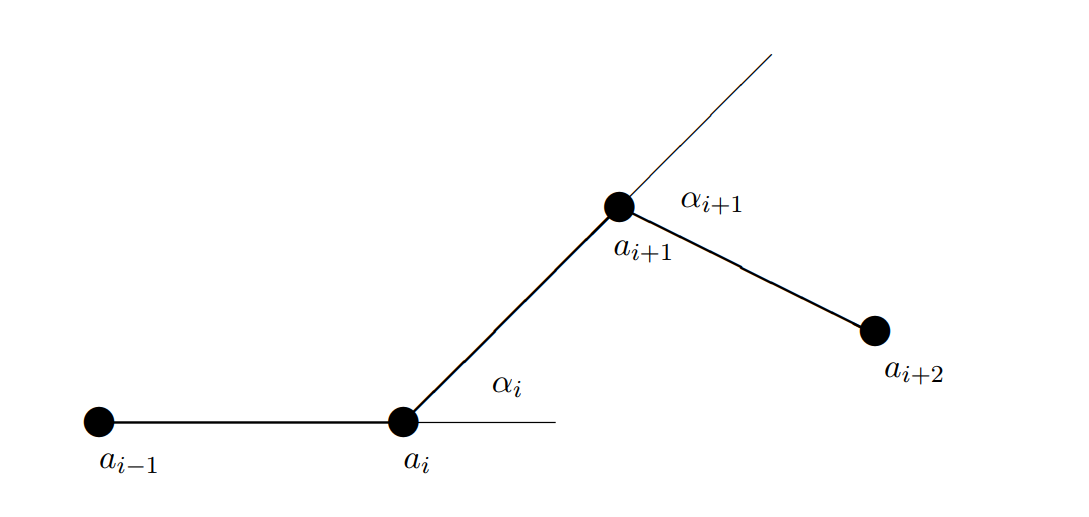
\includegraphics[scale=0.45]{configuration}
        \caption{Problem configuration}
        \label{atom configuration}
    \end{figure}
    
    There are several distinct advantages to this approach compared to using cartesian coordinates:
    \begin{enumerate}
        \item Specifying the angles removes the need to recalculate the positions of atoms after a change (as the angles are relative).
        \item The cartesian coordinates can be obtained for any atom via trigonometry.
        \item The vector of angles is a simpler representation of the problem and the change in energy for the cluster relative to the change in any $\alpha_{i}$ can be determined.
    \end{enumerate}

    
    \clearpage
    \section{Literature Review}
    \subsection{BFGS}
    The Broyden-Fletcher-Goldfarb-Shanno algorithm is an iterative method under the quasi-Newton class of hill climbing algorithms. "Quasi-Newton methods, like steepest descent, require only the gradient of the objective function to be supplied at each iteration" \cite{numericalOptimization}
    The BFGS algorithm will never make a step in the `uphill' direction. To effectively make use of BFGS in problem spaces with local minima BFGS needs to be used as the optimization step in a higher level optimization algorithm such as a genetic population based search.

    \subsection{Cross-Entropy Method}
    The Cross-Entropy method is a generic approach to solving complicated optimization problems such as Max Cut or the travelling salesman problem. "the CE method... defines a precise mathematical frame-work for deriving fast, and in some sense "optimal" updating/learning rules..." \cite{CE}. The core algorithm of the CE method is quite a simple iterative process:
    \begin{enumerate}
        \item Generate a sample of random data according to some mechanism.
        \item Score the sample and take an elite sub sample of the resulting population.
        \item Use the values of the elite sub sample to update the parameters of the random mechanism to produce a "better" sample on the next iteration.
    \end{enumerate}
    The random mechanism can be as simple as specifying a random distribution for each element in the vector to be optimized (in this case the vector of angles) where the mean and standard deviation are changed to reflect the elite sample.
    \\\\
    Specifying a smoothing parameter can be useful \cite{CE2}. The smoothing parameter determines the ratio of change between the old distribution and the newly determined updated distribution. This smoothing parameter $\lambda$ can either be a static value $0 \leq \lambda \leq 1$ or dynamically changed as a function of time, score or another heuristic.

    \clearpage

    \section{Algorithm Description}
    \subsection{Cross Entropy Optimization}
    \subsubsection{Pseudocode}
    \lstinputlisting[language=python]{Code/CE.py}
    
    \clearpage
    \subsection{BFGS and Genetic Search}
    \subsubsection{Pseudocode}
    \lstinputlisting[language=python]{Code/BFGS.py}

    \clearpage
    \subsection{Cross Entropy Method to Generate Optimization Candidates for BFGS}
    \par An experiment to use the Cross Entropy Method as the global optimizer in order to generate optimization candidates for BFGS. Conceptually this method will allow the Cross Entropy Method to optimize the distribution vector to generate good candidates for BFGS optimization.
    \subsubsection{High level algorithm}
    \begin{enumerate}
        \item Generate Population using distribution vector.
        \item Run BFGS on population members, generating an additional optimized population.
        \item Calculate the scores of the optimized population and sort.
        \item Update the distribution vector based on the pre-optimized sequences which correspond to the sequences in the elite sample of the optimized population.
        \item Goto step 1.
    \end{enumerate}
    
    
    % %
    % % ─── EQUILIBRIUM ────────────────────────────────────────────────────────────────
    % %
    % \subsection{Equilibrium}
    % To calculate the equilibrium point of both the predator and prey growth equations the rate of change was set to 0 and then the equation was solved.
    
    % \subsubsection{Equilibrium for Change in Predators}
    % $$ \frac{dN}{dt} = rN - kNP $$
    % $$ 0 = rN - KNP $$
    % $$ 0 = N(r - KP) $$
    % $$ 0 = r - KP $$
    % $$ r = KP $$
    % $$ P = r / K $$
    % $$ P_{Predators} = 0.002 / 0.001 = 2 $$
    
    % \subsubsection{Equilibrium for Change in Prey}
    % $$ \frac{dN}{dt} = -bN - \alpha k NP $$
    % $$ 0 = -bN - \alpha k NP $$
    % $$ 0 = N(-b - \alpha kP) $$
    % $$ 0 = -b - \alpha kP $$
    % $$ b = -\alpha KP $$
    % $$ P = \frac{b}{-\alpha k} $$
    % $$ P_{prey} = \frac{0.001}{0.001 * 0.001} = 1000 $$
    
    % \par
    % The equilibrium results of $P_{Predator} = 2$ $P_{Prey} = 1000$ shows that on average the equilibrium between the two populations will be in the ratio of 2 sharks for every 1000 tuna in the system.
    
    \clearpage
    
    \bibliographystyle{apacite}
    \bibliography{bib}

    \end{document}